\subsection{WYSIWYG}
�WYSIWYG� staat voor �What you see is what you get�. Deze functionaliteit maakt tekst verwerken erg gemakkelijk.

\subsubsection{Koptitels}
\begin{enumerate}
\item Ga met de tekstcursor in de regel staan die een Kop 2 of Kop 3 (subkop) moet worden.
\item Klik op het Opmaak openklapmenu en kies Kop 2 of Kop 3.
\end{enumerate}
Het is niet toegestaan om een heading 1 te gebruiken. Volgens de webrichtlijnen is een Kop 1 altijd de paginatitel en komt deze maar 1 keer voor op een pagina. Het gebruik van koppen in teksten dient echter wel op een juiste manier te gebeuren. Gebruik niet de Vet (Bold) knop maar de Opmaak knop. Voor de hoofdkoppen in de tekst gebruikt u Kop 2. Indien hieronder nog subkoppen gemaakt moeten worden gebruikt u Kop 3.

\begin{center}
	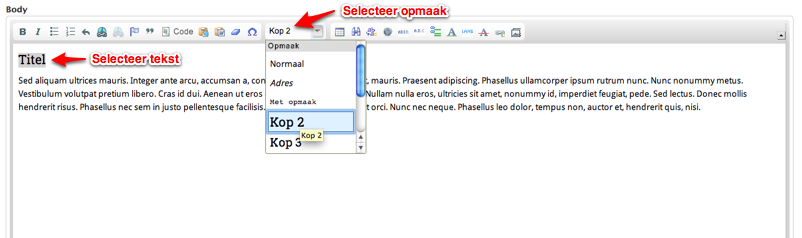
\includegraphics[scale=.7]{img/koptitels.png}
\end{center}

\subsubsection{Bold}
Om een bepaald woord nadruk te geven kan men de Vet (B) knop gebruiken. Gebruik deze knop niet om Headers cq koptitels te maken.
\begin{enumerate}
\item Selecteer het woord met de muis wat u vet wilt maken.
\item Klik op de B-knop.
\item Wilt u het woord niet meer vet hebben, klik dan nog een keer op de B-knop
\end{enumerate}

\begin{center}
	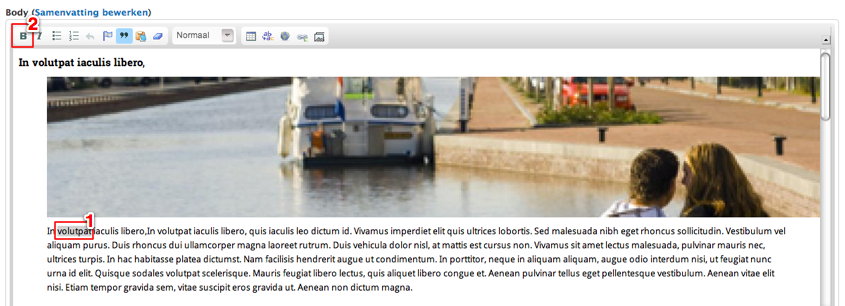
\includegraphics[width=\textwidth]{img/bold.png}
\end{center}

\subsubsection{Italic}
Om een bepaald woord nadruk te geven kan men de Schuin knop gebruiken, oftewel de I-knop.
\begin{enumerate}
\item Selecteer het woord met de muis wat u schuin wilt maken.
\item Klik op de I-knop.	
\item Wilt u het woord niet meer schuingedrukt hebben, klik dan nogmaals op de I-knop.
\end{enumerate}

\begin{center}
	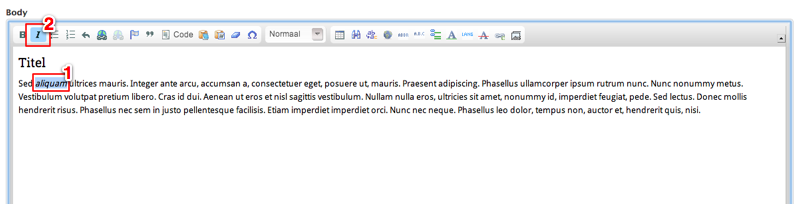
\includegraphics[width=\textwidth]{img/schuin.png}
\end{center}

\subsubsection{Opsomming}
Om een opsomming te maken kan men de Opsomming knop gebruiken.
\begin{enumerate}
\item Klik op de opsomming knop, en voer uw tekst direct in.
\item Om een nieuwe opsommingspunt te gebruiken drukt u op de Enter toets, druk 2 maal op de Enter toets om uit de opsomming te gaan.
\end{enumerate}

\begin{center}
	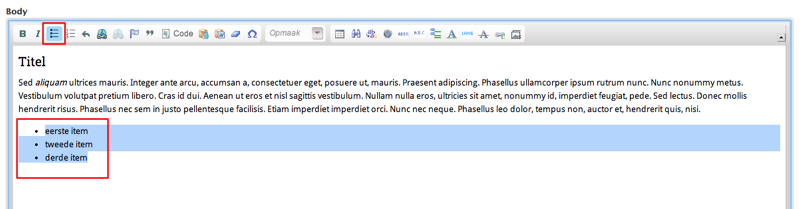
\includegraphics[width=\textwidth]{img/opsomming.png}
\end{center}

\subsubsection{Genummerde lijst}
Om een genummerde lijst te maken kan men de Genummerde lijst knop gebruiken.
\begin{enumerate}
\item Klik op de genummerde lijst knop, en voer uw tekst direct in.
\item Om een nieuw getal te gebruiken drukt u op de Enter toets, druk 2 maal op de Enter toets om uit de genummerde lijst te gaan te gaan.
\end{enumerate}

\begin{center}
	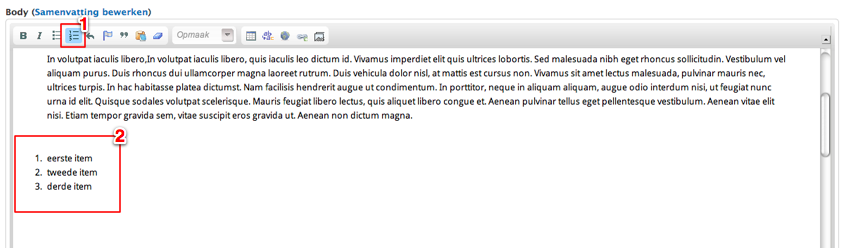
\includegraphics[width=\textwidth]{img/genummerde_lijst.png}
\end{center}

\subsubsection{Afkorting}
Als in de tekst een afkorting wordt gebruikt, bijvoorbeeld maw, dan dient men dit woord te markeren en de betekenis van dit woord te noteren.
\begin{enumerate}
\item Markeer de afkorting.
\item Klik op de Afkorting knop.
\item Noteer de betekenis van de afkorting en druk op OK.
\item U kunt het controleren door met uw muiscursor op het woord te gaan staan.
\end{enumerate}

\begin{center}
	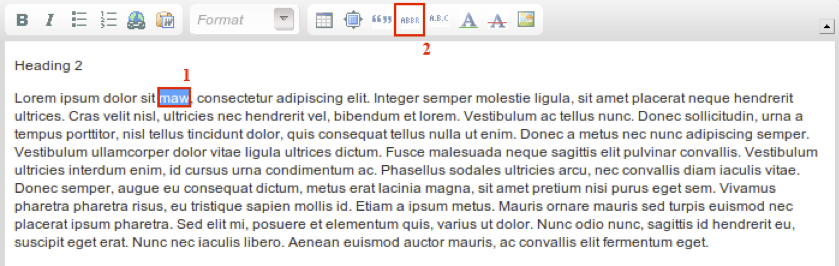
\includegraphics[width=\textwidth]{img/afkorting.png}
	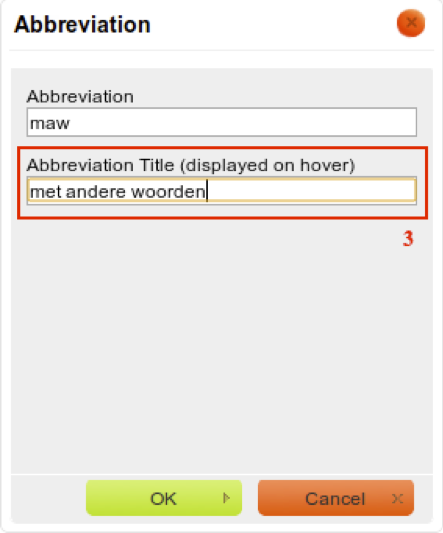
\includegraphics[scale=1]{img/afkorting-1.png}
\end{center}

Let op: Als een afkorting meerdere keren voorkomt in de pagina, dient men alleen de betekenis van de eerste afkorting te noteren.

\subsubsection{Acroniem}
\begin{enumerate}
\item Markeer de acroniem.
\item Klik op de Acroniem knop.
\item Noteer de betekenis van de acroniem en druk op OK.
\item U kunt het controleren door met uw muiscursor op het woord te gaan staan.
\end{enumerate}

\begin{center}
	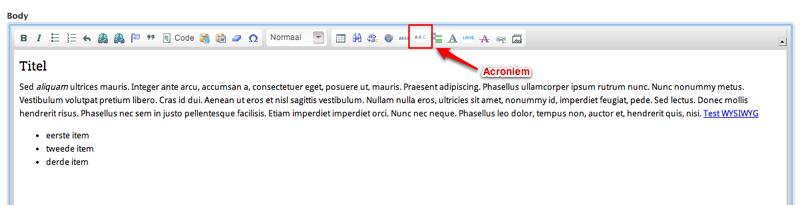
\includegraphics[width=\textwidth]{img/acroniem.png}
	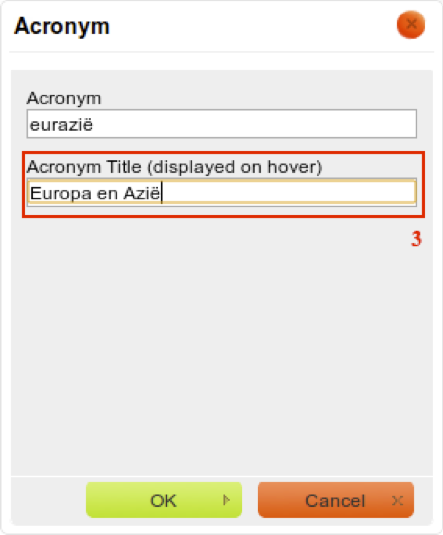
\includegraphics[scale=1]{img/acroniem-1.png}
\end{center}

\subsubsection{Toevoeging en verwijdering}
Op sommige pagina�s is het van belang dat men ziet welke woorden of zinnen er zijn toegevoegd of verwijderd. Dit kan men doen door middel van de Toevoeging knop en de Verwijdering knop.
\begin{center}
	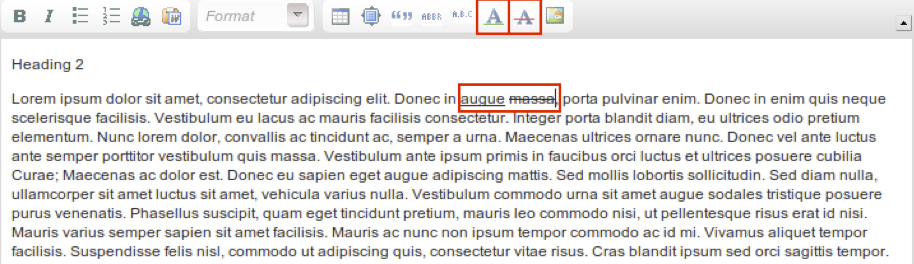
\includegraphics[width=\textwidth]{img/toevoeging-verwijdering.png}
\end{center}

\subsubsection{Citaat}
De Citaat knop wordt gebruikt voor referenties naar personen en titels.
\begin{enumerate}
\item Markeer het betreffende woord.
\item Klik op de Citaat knop
\end{enumerate}

\begin{center}
	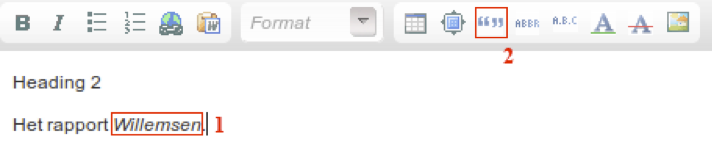
\includegraphics[scale=1]{img/citaat.png}
\end{center}

\subsubsection{Externe links openen automatisch in een nieuw venster}
Via de Extlink module zorgen we ervoor dat links naar andere sites of documenten in een nieuw venster worden geopend.
\begin{center}
	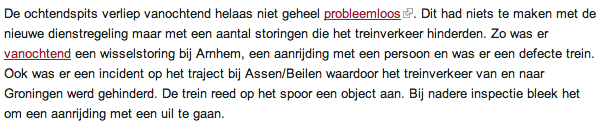
\includegraphics[scale=1]{img/extlink.png}
\end{center}

\subsubsection{Iframes}
Om een andere website te tonen op de ProRail website maken we gebruik van een iframe. Via de wereldbolknop in 
de WYSIWYG kan dit toevoegen aan de pagina. Er zijn drie velden verplicht:
\begin{enumerate}
\item URL
\item Breedte
\item Hoogte
\end{enumerate}

\begin{center}
	
\includegraphics[scale=0.5]{img/iframe1.png}
	De iframe knop in WYSIWYG
\end{center}
\begin{center}
	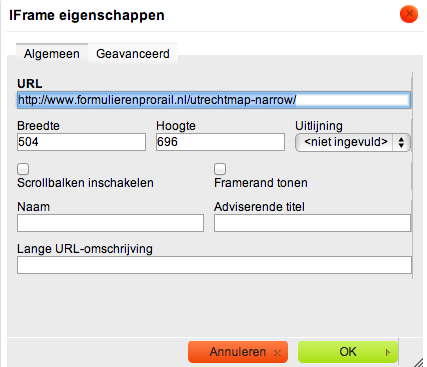
\includegraphics[scale=0.5]{img/iframe2.png}
	Het iframe dialoog
\end{center}
\begin{center}
	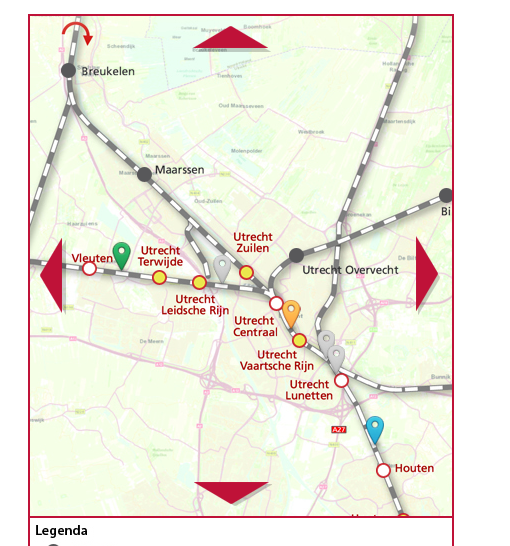
\includegraphics[scale=0.5]{img/iframe3.png}
	Het resultaat
\end{center}

\subsubsection{Tabellen}
Via de tabel knop kan een tabel worden ingevoegd. Via de dropdown koppen kan gekozen worden of de rij of kolom of beide.
\begin{center}
	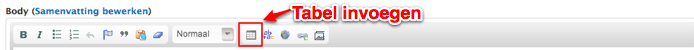
\includegraphics[scale=0.5]{img/tabellen1.png}
\end{center}

\subsubsection{Image Maps}
Image Maps toevoegen gaat op de volgende manier:

\begin{enumerate}
\item Voeg een afbeelding in
\item Rechtermuisknop op de afbeelding en kies Wijzig image map
\item Trek den vierkant of cirkel over het gebied wat klikbaar moet zijn
\item Vul een url in
\item Klik op ok
\end{enumerate}

\begin{center}
	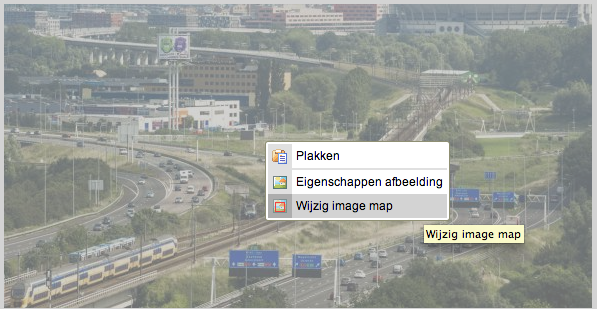
\includegraphics[scale=0.5]{img/imagemap1.png}
	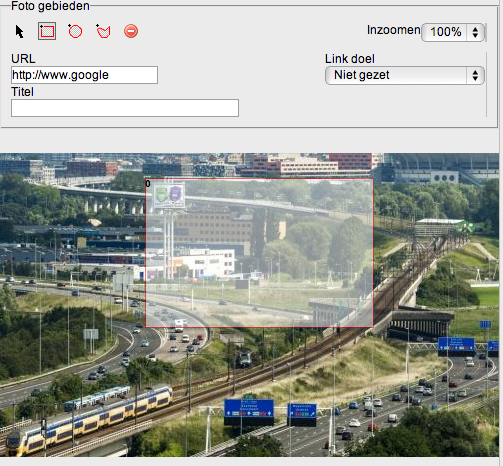
\includegraphics[scale=0.5]{img/imagemap2.png}
\end{center}

\subsubsection{YouTube Embed}
\begin{enumerate}
\item Klik op de media button
\item Vul YouTube url in
\item Kies voor origineel
\end{enumerate}